%%%%%%%%%%%%%%%%%%
% Based on https://github.com/jdavis/latex-homework-template
%%%%%%%%%%%%%%%%%%

\documentclass{article}

\usepackage{fancyhdr}
\usepackage{extramarks}

\usepackage{amsmath}
\usepackage{amsthm}
\usepackage{amsfonts}

\usepackage{tikz}
\usetikzlibrary{matrix}
\usepackage[plain]{algorithm}
\usepackage{algpseudocode}

\usetikzlibrary{automata,positioning, chains}

\usetikzlibrary{positioning, fit, arrows.meta, shapes}

\usepackage{wrapfig}

\usepackage{lipsum}

%for urls
\usepackage{hyperref}
\hypersetup{
	colorlinks = true,
	linkcolor = teal,
	anchorcolor = teal,
	citecolor = teal,
	filecolor = teal,
	urlcolor = teal
}

%for including pdf image
\usepackage{graphicx}

\usepackage{enumerate}

%%%%%% Basic Document Settings %%%%%%%%%

\topmargin=-0.45in
\evensidemargin=0in
\oddsidemargin=0in
\textwidth=6.5in
\textheight=9.0in
\headsep=0.25in

\linespread{1.1}

%%%%%%%%%%%%%%%%%% Homework Details %%%%%%%%%%%%%%%
% University Seal
% Title
% Due date
% University
% Class
% Instructor
% Author
% Author ID 
\newcommand{\hmwkSeal}{images/logo.png}
\newcommand{\hmwkTitle}{Assignment\ \#4}
\newcommand{\hmwkDueDate}{June 30, 2023}
\newcommand{\hmwkClass}{Neural Networks \& Representation Learning (CS-587)}
\newcommand{\hmwkClassInstructor}{Ass. Prof. N. Komontakis}
\newcommand{\hmwkUniversity}{University of Crete \\Department of Computer Science}
\newcommand{\hmwkAuthorName}{Nikolaos Kougioulis}
\newcommand{\hmwkAuthorID}{ID 1285}

%fancyhdr
\pagestyle{fancy}
\lhead{\hmwkAuthorName\ (\hmwkAuthorID)} %left head
%\chead{\hmwkClass\ \hmwkTitle} %center head
%\rhead{\date{\today}} %right head
\rhead{\hmwkClass\ \hmwkTitle} 
\lfoot{\lastxmark}
\cfoot{\thepage}

\renewcommand\headrulewidth{0.4pt}

% Create Problem Sections %

\newcommand{\enterProblemHeader}[1]{
	\nobreak\extramarks{}{Problem \arabic{#1} continued on next page\ldots}\nobreak{}
	\nobreak\extramarks{Problem \arabic{#1} (continued)}{Problem \arabic{#1} continued on next page\ldots}\nobreak{}
}

\newcommand{\exitProblemHeader}[1]{
	\nobreak\extramarks{Problem \arabic{#1} (continued)}{Problem \arabic{#1} continued on next page\ldots}\nobreak{}
	\stepcounter{#1}
	\nobreak\extramarks{Problem \arabic{#1}}{}\nobreak{}
}

\setcounter{secnumdepth}{0}
\newcounter{partCounter}
\newcounter{exerciseCounter}
\setcounter{exerciseCounter}{1}
\nobreak\extramarks{Problem \arabic{exerciseCounter}}{}\nobreak{}

% Homework Problem Environment %
% This environment takes an optional argument. When given, it will adjust the problem counter. This is useful for when the problems given for your
% assignment aren't sequential. See the last 3 problems of this template for an example.
%

\newcommand{\enterExerciseHeader}[1]{
	\nobreak\extramarks{}{Exercise \arabic{#1} continued on next page\ldots}\nobreak{}
	\nobreak\extramarks{Exercise \arabic{#1} (continued)}{Exercise \arabic{#1} continued on next page\ldots}\nobreak{}
}

\newcommand{\exitExerciseHeader}[1]{
	\nobreak\extramarks{Exercise \arabic{#1} (continued)}{Exercise \arabic{#1} continued on next page\ldots}\nobreak{}
	\stepcounter{#1}
	\nobreak\extramarks{Exercise \arabic{#1}}{}\nobreak{}
}

\newenvironment{Exercise}[1][-1]{
	\ifnum#1>0
	\setcounter{exerciseCounter}{#1}
	\fi
	\section{Exercise \arabic{exerciseCounter}}
	\setcounter{partCounter}{1}
	\enterExerciseHeader{exerciseCounter}
}{
	\exitExerciseHeader{exerciseCounter}
}

% Title Page %
\title{
	\centering
	\includegraphics[height=1.5in]{\hmwkSeal}
	
	\vspace{1in}
	\textmd{\textbf{\hmwkClass\ \hmwkTitle}}\\
	
	\normalsize\vspace{0.1in}\small{Due\ on\ \hmwkDueDate}\\
	
	\vspace{0.1in}
	\large{\textit{\hmwkClassInstructor}} \\
	\vspace{0.5in}
	
	\large{\hmwkUniversity}
	
	\vspace{3in}
	
	\author{\textbf{\hmwkAuthorName} (\hmwkAuthorID)}
	\date{\today}
}

% Various Helpers %
\newcommand{\alg}[1]{\textsc{\bfseries \footnotesize #1}}
% For derivatives
\newcommand{\deriv}[1]{\frac{\mathrm{d}}{\mathrm{d}x} (#1)}
% For partial derivatives
\newcommand{\pderiv}[2]{\frac{\partial}{\partial #1} (#2)}
% Integral dx
\newcommand{\dx}{\mathrm{d}x}
\newcommand{\E}{\mathbb{E}}
\newcommand{\Var}{\mathrm{Var}}
\newcommand{\Cov}{\mathrm{Cov}}
\newcommand{\Bias}{\mathrm{Bias}}
\newcommand{\Prob}{\mathbb{P}}

\def\code#1{\texttt{#1}}

%for code listings
\usepackage{listings}
\usepackage{xcolor}

\definecolor{codegreen}{rgb}{0,0.6,0}
\definecolor{codegray}{rgb}{0.5,0.5,0.5}
\definecolor{codepurple}{rgb}{0.58,0,0.82}
\definecolor{backcolour}{rgb}{0.99,0.99,0.99}

\lstdefinestyle{mystyle}{
	backgroundcolor=\color{backcolour},   
	commentstyle=\color{codegreen},
	keywordstyle=\color{magenta},
	numberstyle=\tiny\color{codegray},
	stringstyle=\color{codepurple},
	basicstyle=\ttfamily\footnotesize,
	breakatwhitespace=false,         
	breaklines=true,                 
	captionpos=b,                    
	keepspaces=true,                 
	numbers=left,                    
	numbersep=5pt,                  
	showspaces=false,                
	showstringspaces=false,
	showtabs=false,                  
	tabsize=2
}

\lstset{style=mystyle}

\begin{document}
	
	\maketitle
	
	\pagebreak
	
\section{Part A: RNN cells}

For the first part of the programming assignment, the task is to implement an RNN cell and an RNN model. 

\begin{figure}[h]
	\centering
	\includegraphics[width=0.8\textwidth]{images/RNN_cell_forward.png}
	\caption{Illustration of the given RNN cell.}
\end{figure}

\begin{enumerate}
	\item At this step we have to implement the forward step of the RNN cell illustrated in Figure 1. We compute the hidden state $a^{\langle t \rangle}$ (substep 1), which is the output of the RNN cell in the figure, compute the prediction \code{yt\_pred} $\hat{y}^{\langle t \rangle}$ (substep 2) and then return the tuple $(a^{\langle t \rangle} , a^{\langle t \rangle} , x^{\langle t \rangle}, \text{parameters})$ as a python tuple (substep 3). This is illustrated in the code snippet below: \\
	 
	\begin{lstlisting}[language=Python]
	# 1. compute next activation state using the formula in the RNN cell figure
	
	a_next = np.tanh(np.dot(Waa, a_prev) + np.dot(Wax, xt) + ba)
	
	# 2. compute output of the current cell using the formula given above   
	
	yt_pred = softmax(np.dot(Wya, a_next) + by) 
	
	# 3. store values you need for backward propagation in cache
	
	cache = (a_next, a_prev, xt, parameters)\end{lstlisting}
	\item We now need to fill-in the \code{rnn\_forward} function to implement the forward pass of the model. We create two arrays $a$ and $y$ of zeros with shape $(n_a , m, T_x )$ for storing the hidden states and $(n_y , m, T_x )$ respectively that will store the predictions (substep 1).

\begin{lstlisting}[language=Python]
	a, y_pred = np.zeros((n_a, m, T_x)), np.zeros((n_y, m, T_x))\end{lstlisting}

    \item We initialize the 2-dimensional hidden state $a_{next}$ by setting it equal to the initial hidden state $a_0$ simply by \code{a\_{next} = a\_0} (substep 2).
    
    \item For the next step, again in the forward pass function, we begin by iterating through every timestep $T_x$ (first line of code snippet). We obtain the data to be fed to the RNN cell as a slice of x, with x having a shape of $(n_x , m, Tx )$ and update the hidden state by calling the \code{rnn\_cell\_forward} function and storing the next hidden state and currect $\hat{y}^{\langle t \rangle}$ prediction. Values are then appended to the list of cache for the backward pass.
    
    \begin{lstlisting}[language=Python]
    for t in range(T_x):
        a_next, yt_pred, cache = rnn_cell_forward(x[:,:,t], a_next, parameters) 
        a[:,:,t], y_pred[:,:,t] = a_next, yt_pred
        caches.append(cache)\end{lstlisting}

\end{enumerate}

Testing the given input (hidden states and predictions) and output, it appears everything works as expected: \code{a[4][1] = [-0.99999375  0.77911235 -0.99861469 -0.99833267]},
\code{y\_pred[1][3] = [0.79560373 0.86224861 0.11118257 0.81515947]}.

\begin{figure}
	\centering
	\includegraphics[width=1.0\textwidth]{images/RNN_sequence_of_cells.png}
	\caption{Illustration of the complete RNN model.}
\end{figure}

\begin{itemize}
	\item \textbf{Question A:} Explain briefly the general functionality of RNN cells (how do we achieve memorization, the purpose of each function on the memorization task). \\
	
	\textbf{Answer:} The general functionality of RNN cells is to process sequential data by maintaining and utilizing information from previous steps or time points. In more detail, an RNN cell is define by a hidden state function $$h_t = \phi(x_t, h_{t-1};w)$$ and a prediction function $y_t = \psi(h_t;w)$ where $h_t \in \mathbb{R}^Q, ~x_t \in \mathbb{R}^D$ and $w$ the parameters. For instance, \textit{Elman Networks} are of the form
	
	$$ h_t = \phi (W_{h} x_t + U_{h} y_{t-1} + b_h) $$
	$$ y_t = \psi (W_{y} h_t + b_y) $$
	
	where $x_t$ represents the input vector, $h_t$ the hidden layer vector, $y_t$ the output vector, $W,U$ and $b$ are the parameter matrices and parameter vectors respectively and $\phi,\psi$ the (non-linear) activation functions. \\
	
	To better understand the model, the feedback loop of the RNN cell is \textit{unrolled}, with the length of the unrolled cell being equal to the number of time steps of the input sequence (Figure 3). \\
	
	Memorization is evident by observing the underlying temporal dependencies in the formulas of the RNN cell, as well as the illustration of the unrolled model. The hidden state of the unfolded network is formed by incorporating previous observations of the input sequence. Within each cell, the current input $x$, the previous hidden state $h$ and a bias $b$ are combined and transformed by a (non-linear) activation function to determine the current hidden state.
	
	%\iffalse
	
	\begin{figure}[h!]
		\centering
		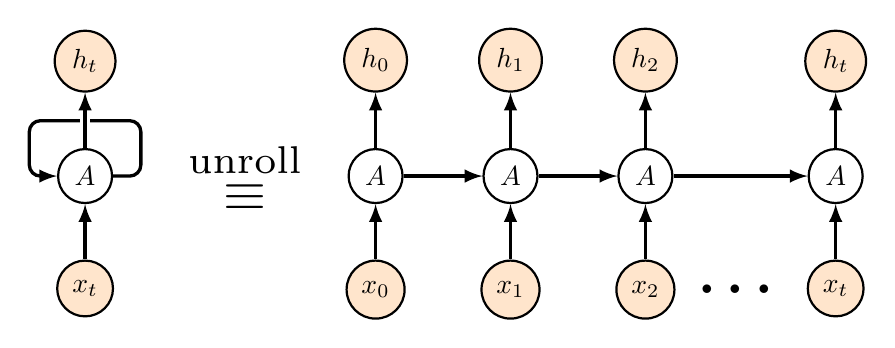
\begin{tikzpicture}[item/.style={circle,draw,thick,align=center},
			itemc/.style={item,on chain,join}]
			\begin{scope}[start chain=going right,nodes=itemc,every
				join/.style={-latex,very thick},local bounding box=chain]
				\path node (A0) {$A$} node (A1) {$A$} node (A2) {$A$} node[xshift=2em] (At)
				{$A$};
		    \end{scope}
	    \node[left=1em of chain,scale=2] (eq) {$\stackrel{\text{unroll}}{\equiv}$
	    };
		\node[left=2em of eq,item] (AL) {$A$};
		\path (AL.west) ++ (-1em,2em) coordinate (aux);
		\draw[very thick,-latex,rounded corners] (AL.east) -| ++ (1em,2em) -- (aux) 
		|- (AL.west);
		\foreach \X in {0,1,2,t} 
		{\draw[very thick,-latex] (A\X.north) -- ++ (0,2em)
			node[above,item,fill=orange!20] (h\X) {$h_\X$};
			\draw[very thick,latex-] (A\X.south) -- ++ (0,-2em)
			node[below,item,fill=orange!20] (x\X) {$x_\X$};}
		\draw[white,line width=0.8ex] (AL.north) -- ++ (0,1.9em);
		\draw[very thick,-latex] (AL.north) -- ++ (0,2em)
		node[above,item,fill=orange!20] {$h_t$};
		\draw[very thick,latex-] (AL.south) -- ++ (0,-2em)
		node[below,item,fill=orange!20] {$x_t$};
		\path (x2) -- (xt) node[midway,scale=2,font=\bfseries] {\dots};
	\end{tikzpicture}
    \caption{Unfolding a recurrent neural network. The length of the unrolled cell is equal to the time steps of the input sequence.}
    \end{figure}

    %\fi
	
	\item \textbf{Question B:} List the limitations of RNNs, as well as try to briefly mention why these issues arise. \\

	\textbf{Answer:} Limitations of RNNs include\footnote{Karpathy, Andrej. "The Unreasonable Effectiveness of Recurrent Neural Networks." Andrej Karpathy blog, May 21, 2015. \url{https://karpathy.github.io/2015/05/21/rnn-effectiveness/} (accessed May 15, 2023).}:
	
	\begin{itemize}
		\item Vanishing/Exploding Gradient Problem: RNNs suffer from difficulties in learning long-term dependencies due to the vanishing or exploding gradient problem. When gradients become too small or too large during backpropagation, it becomes challenging for the network to propagate useful information across long sequences. \\
		
		This can be illustrated using a "vanilla" RNN model. The basic formulation of a vanilla RNN block is the following: $$h_t = \tanh (W_h h_{t-1} + W_x x_t + b) ~\forall t=1,2,\ldots$$
	
	    Notice that the matrices $W_h, W_x$ and the bias $b$ are independent of $t$ which means they are parameters shared across all timestamps of the RNN model. Without loss of generality, considering $h_t$ and $x_t$ to be scalar values, the gradient, which is necessary for back-propagation, of the output $h_t$ with respect to $W_h$ is
	        
	    \begin{equation}
	    	\nabla_{W_h}(h_t) = \text{tanh}^\prime(W_h h_{t-1} + W_x x_t + b) \cdot \frac{\partial (W_h h_{t-1} + W_x x_t + b)}{\partial W_h}
	    \end{equation}
    
        with 
	    \begin{equation}
	    	\frac{\partial (W_h h_{t-1} + W_x x_t + b)}{\partial W_h} = h_{t-1} + W_h \cdot \frac{\partial h_{t-1}}{\partial W_h} \, .
	    \end{equation}
	    
	    The form of a previous timestamp $\displaystyle \frac{\partial h_{t-1}}{\partial W_h}$ will be similar to the one of $\nabla_{W_h}(h_t)$ and  after letting $W_h h_{t-1} + W_x x_t + b \equiv f_t$ we obtain:
	    
	    \begin{eqnarray}
	    	\nabla_{W_h}(h_t) &=& \tanh^\prime(f_t) \cdot
	    	\left(
	    	h_{t-1} + W_h \cdot \frac{\partial h_{t-1}}{\partial W_h}
	    	\right) \\
	    	&=& \tanh^\prime(f_t) \cdot
	    	\left(
	    	h_{t-1} + W_h \cdot \tanh^\prime(f_{t-1}) \cdot
	    	\left(
	    	h_{t-2} + W_h \cdot \left( \dots \right)
	    	\right)
	    	\right) \\
	    	&=& h_{t-1} \tanh^\prime(f_t) + h_{t-2} W_h \tanh^\prime(f_t) \text{tanh}^\prime(f_{t-1}) + \dots \\
	    	&=& \sum_{t^\prime = 1}^{t-1} h_{t^\prime} \left( W_h^{t-t^\prime-1} \tanh^\prime(f_{t^\prime+1}) \cdot \cdots \cdot \tanh^\prime(f_{t}) \right)
	    \end{eqnarray}
	    
	    In other words, the influence of $h_{t^\prime}$ will be mitigated by a factor
	    $W_h^{t-t^\prime-1} \tanh^\prime(f_{t^\prime+1}) \cdot \cdots \cdot  \tanh^\prime(f_{t})$. 
	    
	    Since $\left( \tanh x \right)^\prime = 1 - \tanh ^2 x$, the whole expression will result highly close to zero (thus vanish, See \footnote{Romain Tavenard, Deep Learning Lecture Notes, Université de Rennes 2. Available at \url{https://rtavenar.github.io/deep_book/book_en.pdf}}). The above expression makes clear of the limited ability of RNNs to remember long term dependencies from past steps in the sequence. As the length of the input increases, the ability to retain information from earlier steps vanishes.

	    \item Another limitation of recurrent neural network architectures is the lack of parallelism. Information is processed in a sequential and serial manner, through a series of repeated layers, thus making training and inference slower. The sequential order of the execution inspired the introduction of the Attention mechanism and the transformers architecture that take the whole input sequence at once. Quoting from the 2017 paper\footnote{Vaswani, A., Shazeer, N., Parmar, N., Uszkoreit, J., Jones, L., Gomez, A. N., ... \& Polosukhin, I. (2017). \textit{Attention Is All You Need}. Advances in Neural Information Processing Systems, 30. Preprint available at \url{https://arxiv.org/pdf/1706.03762.pdf}} of Vaswani, Shazeer et. al: \\
	    
	    \begin{quote}
	    \textit{
	    	Recurrent models typically factor computation along the symbol positions of the input and output sequences. Aligning the positions to steps in computation time, they generate a sequence of hidden states $h_t$ as a function of the previous hidden state $h_{t-1}$ and the input for position $t$. This inherently sequential nature precludes parallelization within training examples, which becomes critical at long sequence lengths, as memory constraints limit batching across examples.
	    }
	    \end{quote}
	
	\end{itemize}

	These issues that arise in practice can be handled by GRUs (Gated Recurrent Units) and Long Short Term Memory (LSTM) cells \footnote{Xiao, Fanyi,. "Deep Neural Networks Basics" ECS 289G - Visual Recognition, Computer Science Department at UC Davis \url{https://web.cs.ucdavis.edu/~yjlee/teaching/ecs289g-fall2016/DNN.pdf} (accessed June 2, 2023)}.
	
	\begin{figure}
		\centering
		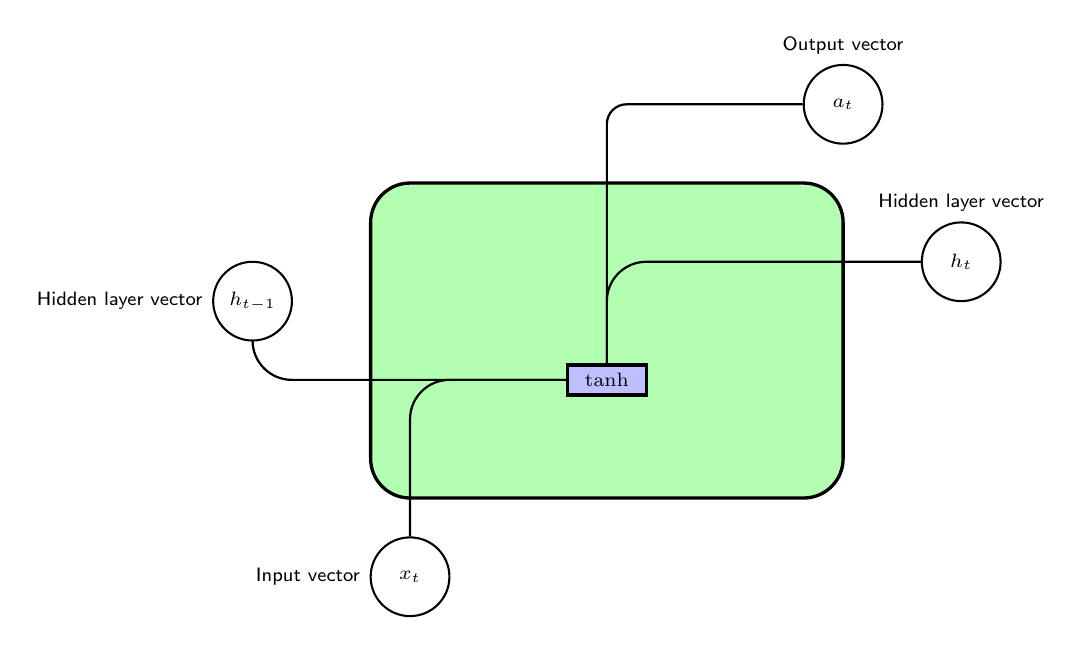
\begin{tikzpicture}[
			% GLOBAL CFG
			font=\sf \scriptsize,
			>=LaTeX,
			% Styles
			cell/.style={% For the main box
				rectangle, 
				rounded corners=5mm, 
				draw=black,
				fill=green!30, % Green fill color
				very thick,
			},
			operator/.style={% For operators like + and x
				circle,
				draw,
				inner sep=-0.5pt,
				minimum height=.2cm,
				fill=yellow!10, % Yellow fill color
				very thick,
			},
			function/.style={% For functions
				ellipse,
				draw,
				inner sep=1pt
			},
			ct/.style={% For external inputs and outputs
				circle,
				draw,
				line width=.75pt,
				minimum width=1cm,
				inner sep=1pt,
			},
			gt/.style={% For internal inputs
				rectangle,
				draw=black,
				minimum width=4mm,
				minimum height=3mm,
				inner sep=3pt,
				fill=blue!25, % Blue fill color
				very thick,
			},
			mylabel/.style={% something new that I have learned
				font=\scriptsize\sffamily
			},
			ArrowC1/.style={% Arrows with rounded corners
				rounded corners=.25cm,
				thick,
			},
			ArrowC2/.style={% Arrows with big rounded corners
				rounded corners=.5cm,
				thick,
			},
			]		
			% Start drawing the thing...    
			% Draw the cell: 
			\node [cell, minimum height=4cm, minimum width=6cm] at (0,0){};
			
			% Draw Internal inputs
			\node [gt, minimum width=1cm] (ibox5) at (0,-0.5) {$\mathbf{\tanh}$};
			
			% Draw External inputs/outputs named as basis c,h,x
			\node[ct, label={[mylabel]left:Hidden layer vector}] (h) at (-4.5,0.5) {$h_{t-1}$};
			\node[ct, label={[mylabel]left:Input vector}] (x) at (-2.5,-3) {$x_{t}$};
			
			% Draw External outputs named as basis c2,h2,x2
			\node[ct, label={[mylabel]Output vector}] (c2) at (3,3) {$a_{t}$};
			\node[ct, label={[mylabel]Hidden layer vector}] (h2) at (4.5,1) {$h_{t}$};
			
			% Drawing arrows
			\draw [-, ArrowC2] (h) |- (ibox5);
			\draw [-, ArrowC2] (x) |- (ibox5);
			\draw [-, ArrowC1] (ibox5) -- (ibox5 |- c2) -- (c2);
			\draw [-, ArrowC2] (ibox5) |- (h2);
			
		\end{tikzpicture}
		
		\caption{Illustration of an rNN cell.}
	\end{figure}
	
	\item \textbf{Question C:} Consider the two following problems, (a) Recognizing images between 10 different species of birds, and (b) Recognizing whether a movie review says that the movie is worth watching or not. For which of the two problems can we use a RNN-based model? Justify your answer. \\
	
	\textbf{Answer:} 
	
	As we have seen in the previous assignment, image recognition is more appropriate to be handled by convolutional neural networks (cNNs). Due to their architecture to capture local characteristics (such as edges) and proceed to capture more global and invariant characteristics at the deepest layers, their handling of hierarchical makes them more suited towards distincting between different species of birds. \\ 
	
	For recognizing whether a movie review says that the movie is worth watching or not, RNN models (and their variations) are an appropriate option. Since movie reviews are written in text, this task requires handling sequences of words in order to model their temporal dependencies sequentially over the whole review text.
	
	\item \textbf{Question D:} While training an RNN, you observe an increasing loss trend. Upon looking you find out that at some point the weight values increase suddenly very much and finally, take the value \code{NaN}. What kind of learning problem does this indicate? What can be a solution? (\textbf{HINT:} answer this after you get a glimpse of Part B). \\
	
    \textbf{Answer:} An increasing loss trend followed by weight values suddenly becoming very large and resulting in \code{NaN} indicates weight values that are outside the floating-point range, thus depicts an exploding gradient problem during back-propagation. To combat this one can use gradient clipping (see Part B).
	
	\item \textbf{Question E:} Gated Recurrent Units (GRUs) have been proposed as a solution on a specific problem of RNNs. What is the problem they solve? And how? \\
	
	\textbf{Answer:} As mentioned previously, GRUs\footnote{Cho, Kyunghyun; van Merrienboer, Bart; Bahdanau, DZmitry; Bougares, Fethi; Schwenk, Holger; Bengio, Yoshua (2014). \textit{Learning Phrase Representations using RNN Encoder-Decoder for Statistical Machine Translation}. arXiv:1406.1078.} were introduced as a solution to address the vanishing gradient problem and the challenge of capturing and retaining information of long-term dependencies in traditional RNNs. \\
	
	GRUs introduce gating mechanisms that regulate the flow of information within the recurrent units. They incorporate two main gates: the update gate and the reset gate. These gates control the flow of information from the previous hidden state and the current input to the current hidden state.
	
	For a fully gated unit, initially, for $t = 0$ the output vector is $h_0 = 0$. Then
	\begin{align*}
		z_t &= \sigma(W_{z}\cdot [h_{t-1},x_t] \\
		r_t &= \sigma(W_{r}\cdot [h_{t-1},x_t] \\
		\tilde{h}_t &= \tanh (W \cdot [r_t \odot h_{t-1},x_t] \\
		h_t &=   (1-z_t) \odot h_{t-1} + z_t \odot  \tilde{h}_t 
\end{align*}

where we have two types of gates, an update gate and a reset gate (A GRU is like a long short-term memory (LSTM) with a forget gate but with fewer parameters than an LSTM, as it lacks the output gate.). The update gate determines the amount of information to be retained from the previous state, and the reset gate the amount of information to be ignored from the previous hidden state when computing the current hidden state. Variations exist, such as the minimal gated unit and the light gated recurrent unit, in the way they implement the gating (e.g the minimal gated unit merges the update and reset gate to a forget gate). \\

	\begin{figure}
		\centering
		\includegraphics[width=0.6\textwidth]{images/Gated_Recurrent_Unit_base_type.png}
	    \caption{Illustration of a Fully Gated GRU cell.}
	\end{figure}

The above allow GRUs to retain and update information from previous timesteps in a selective manner, thus effectively capturing both short-term and long-term dependencies, controlling the flow of information much more robustly than traditional RNNs.
	
\end{itemize}

\pagebreak

\section{Part B}

For the second part of the assignment, as an application of the RNN model that was implemented in the previous part of the assignment, we will use it to build a character level language model to generate new text, more precisely generating chemical element names and then movie names. \\

We specify the corresponding path of the text file containing known chemical names using the \code{os} library, \code{path\_data = os.path.join('data','element\_list.txt')}. \\

From the provided list of element names, the splitting results in 25 characters, including spaces, special characters and the newline character, to form the chemical names. The complete RNN model handling the characters is illustrated in Figure 2. At each step, the RNN tries to predict the next candidate character. The given dataset $X = (x^{\langle 1 \rangle}, x^{\langle 2 \rangle}, ..., x^{\langle T_x \rangle})$ corresponds to the list of characters in the training set, while $Y = (y^{\langle 1 \rangle}, y^{\langle 2 \rangle}, ..., y^{\langle T_x \rangle})$ is such that at every time-step $t$, we have $y^{\langle t \rangle} = x^{\langle t+1 \rangle}$ (see the provided comments at the accompanied \code{.ipynb} notebook). \\

Regarding the coding pipeline, after loading the text file and obtaining the unique characters, we must define the forward and backward operations for constructing the model. As mentioned before, gradient clipping is utilized, leading us to answer the following questions:

\begin{itemize}
	\item \textbf{Question A:} What is the purpose of gradient clipping? What learning limitation we are aiming to solve? \\
	
	\textbf{Answer:} The purpose of gradient clipping is to address the exploding gradient problem during the training of deep neural networks, particularly recurrent neural networks (RNNs). Gradient clipping is a technique that constraints the numerical magnitude of the gradients during back-propagation within an imposed threshold, preventing them from becoming too large \footnote{\url{https://angelina-yang.medium.com/what-is-gradient-clipping-d676eeaeb294}} and thus facilitating the learning process. The exploding gradient problem can result in divergence from a local maxima and unstable training and as seen before, in extreme cases can lead to \code{NaN} weight values.
	
\end{itemize}

Following the rest of the guidelines for the coding pipeline, we have: \\

For the \code{rrn\_step\_forward} function, we define the operations for the hidden state and the prediction for every time step, as shown in Figure 1. For the backward step, in \code{rrn\_step\_backward}, the partial derivatives are computed for each of the parameters $dWya, dby, da_next, db, dWax, dWaa, da_next$ and stored in a python dictionary. The gradients of this step are then used on \code{update\_parameters} to define the updates for the parameters of the RNN cell from gradient descent, stored in a dictionary too and returned by the function. Gradient clipping is then implemented in the \code{clip} function by iterating with a \code{for} loop over the gradients of each parameter using \code{np.clip}\footnote{\url{https://numpy.org/doc/stable/reference/generated/numpy.clip.html}}. \\

Finally, in the \code{optimize} functions, by calling the appropriate functions according to the provided comments, we perform a forward pass through time, then a backward pass, perform gradient clipping for absolute values over 5 and update the parameters, using the functions we have filled before.

	\begin{figure}[h]
	\centering
	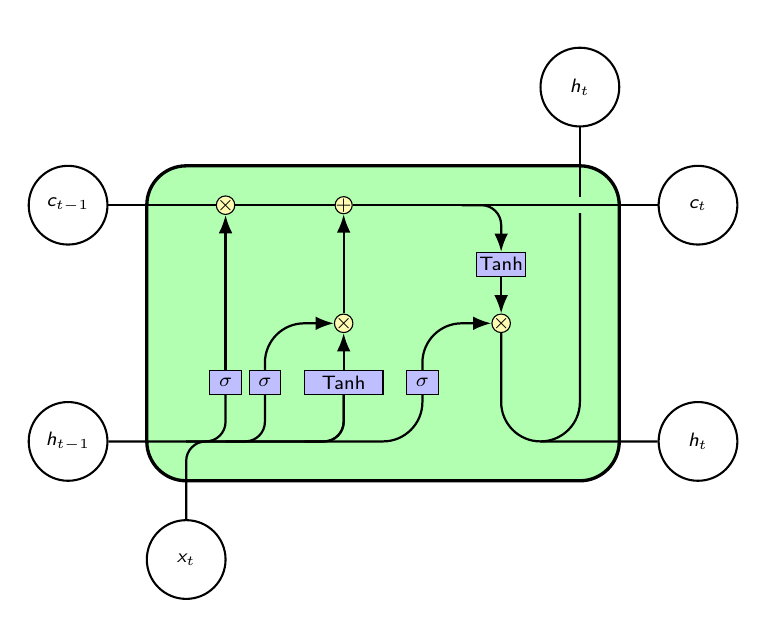
\begin{tikzpicture}[
		% GLOBAL CFG
		font=\sf \scriptsize,
		>=LaTeX,
		% Styles
		cell/.style={% For the main box
			rectangle, 
			rounded corners=5mm, 
			draw,
			fill=green!30,
			very thick,
		},
		operator/.style={%For operators like +  and  x
			circle,
			draw,
			fill=yellow!30,
			inner sep=-0.5pt,
			minimum height =.2cm,
		},
		function/.style={%For functions
			ellipse,
			draw,
			inner sep=1pt
		},
		ct/.style={% For external inputs and outputs
			circle,
			draw,
			line width = .75pt,
			minimum width=1cm,
			inner sep=1pt,
		},
		gt/.style={% For internal inputs
			rectangle,
			draw,
			fill=blue!25,
			minimum width=4mm,
			minimum height=3mm,
			inner sep=1pt
		},
		mylabel/.style={% something new that I have learned
			font=\scriptsize\sffamily
		},
		ArrowC1/.style={% Arrows with rounded corners
			rounded corners=.25cm,
			thick,
		},
		ArrowC2/.style={% Arrows with big rounded corners
			rounded corners=.5cm,
			thick,
		},
		]		
		%Start drawing the thing...    
		% Draw the cell: 
		\node [cell, minimum height =4cm, minimum width=6cm] at (0,0){} ;
		
		% Draw inputs named ibox#
		\node [gt] (ibox1) at (-2,-0.75) {$\sigma$};
		\node [gt] (ibox2) at (-1.5,-0.75) {$\sigma$};
		\node [gt, minimum width=1cm] (ibox3) at (-0.5,-0.75) {Tanh};
		\node [gt] (ibox4) at (0.5,-0.75) {$\sigma$};
		
		% Draw opérators   named mux# , add# and func#
		\node [operator] (mux1) at (-2,1.5) {$\times$};
		\node [operator] (add1) at (-0.5,1.5) {+};
		\node [operator] (mux2) at (-0.5,0) {$\times$};
		\node [operator] (mux3) at (1.5,0) {$\times$};
		\node [gt] (func1) at (1.5,0.75) {Tanh};
		
		% Draw External inputs? named as basis c,h,x
		\node[ct, label={[mylabel]}] (c) at (-4,1.5) {$\emph{c}_{t-1}$};
		\node[ct, label={[mylabel]}] (h) at (-4,-1.5) {$\emph{h}_{t-1}$};
		\node[ct, label={[mylabel]}] (x) at (-2.5,-3) {$\emph{x}_{t}$};
		
		% Draw External outputs? named as basis c2,h2,x2
		\node[ct, label={[mylabel]}] (c2) at (4,1.5) {$\emph{c}_{t}$};
		\node[ct, label={[mylabel]}] (h2) at (4,-1.5) {$\emph{h}_{t}$};
		\node[ct, label={[mylabel]}] (x2) at (2.5,3) {$\emph{h}_{t}$};
		
		% Start connecting all.
		%Intersections and displacements are used. 
		% Drawing arrows    
		\draw [ArrowC1] (c) -- (mux1) -- (add1) -- (c2);
		
		% Inputs
		\draw [ArrowC2] (h) -| (ibox4);
		\draw [ArrowC1] (h -| ibox1)++(-0.5,0) -| (ibox1); 
		\draw [ArrowC1] (h -| ibox2)++(-0.5,0) -| (ibox2);
		\draw [ArrowC1] (h -| ibox3)++(-0.5,0) -| (ibox3);
		\draw [ArrowC1] (x) -- (x |- h)-| (ibox3);
		
		% Internal
		\draw [->, ArrowC2] (ibox1) -- (mux1);
		\draw [->, ArrowC2] (ibox2) |- (mux2);
		\draw [->, ArrowC2] (ibox3) -- (mux2);
		\draw [->, ArrowC2] (ibox4) |- (mux3);
		\draw [->, ArrowC2] (mux2) -- (add1);
		\draw [->, ArrowC1] (add1 -| func1)++(-0.5,0) -| (func1);
		\draw [->, ArrowC2] (func1) -- (mux3);
		
		%Outputs
		\draw [-, ArrowC2] (mux3) |- (h2);
		\draw (c2 -| x2) ++(0,-0.1) coordinate (i1);
		\draw [-, ArrowC2] (h2 -| x2)++(-0.5,0) -| (i1);
		\draw [-, ArrowC2] (i1)++(0,0.2) -- (x2);
		
	\end{tikzpicture}
	\caption{Illustration of an LSTM Cell.}
\end{figure}

\begin{itemize}
	
	\item \textbf{Question B:} What do you observe about the new generated chemical names? How do you interpret the format of the new generated chemical element names? \\
	
	\textbf{Answer:} We run the model for 100k iterations, 7 samples at each iteration, 65 units at each RNN cell, with a learning rate of 0.01. Every 2000 iterations generated characters are printed. Notice that during the first iterations, the generated names do not make much sense, for example
	
\begin{lstlisting}
Iteration: 0, Loss: 22.538572
		
Nkzxwucmeroeygtrw
Knea
Kzxwucmeroeygtrw
Nea
Zxwucmeroeygtrw
Ea
Xwucmeroeygtrw\end{lstlisting} 

    But as the loss gets lower, many generated names at the final iterations are plausible candidates for naming an unknown element (probably an element not found to occur naturally on Earth), for instance
    
\begin{lstlisting}
Iteration: 98000, Loss: 10.196881
    
Potponium
Nohodium
Nopsenchordonium
Pelaerium
Totabtinum
Leaburm
Totabtunum\end{lstlisting}
    
    Notice how the names of the elements end in "um" "-ium" etc, since these are the final characters found in most elements provided in our test data. 
    
    \item \textbf{Question C:} What happens when you train your model for the movie titles dataset? what do you observe and how do you interpret this observation?\\
	
	\textbf{Answer:}
	
	In order to train our model for the movie titles, we notice that instead of 25 we have 42 unique characters in our data, and as such must modify our code accordingly (see comments on the notebook): The parameter \code{vocab\_size} when performing the forward pass in the function \code{rnn\_forward} and when training the model in the function \code{model}, to accommodate for the new dimensions of the tensors. \\
	
	As before, for 60k iterations, 10 samples at each iteration, 30 units at each RNN cell, with a learning rate of 0.01, at the first iterations it generates random names, and at the final iterations more plausible movie names, like the following:
	
	\begin{lstlisting}
	Iteration: 68000, Loss: 34.098450
		
	Onyiss of the spuathers alory lamans
	Inca
	Istrgand of the blandes
	On -axse berro javen
	The eplk grapis
	Ca
	The park
	A
	The greaundes
	Aity a prathersa fuperteior die the larna the poce\end{lstlisting}
    
    Observe that the generated titles and "creativity" is limited to the provided list of movies, more specifically the words and phrases that appear more frequently and hence the generated titles do not always produce meaningful or plausible movie titles. Some generated names are definetely candidates for a possible movie, such as "The park", "Inca" and "Istrgrand of the blandes" (a name for a Norwegian movie about Black Metal perhaps?). This is obviously a more complex task than the previous one, as it involves more complex names and more words.
	
	\item \textbf{Question D:} Can you think of ways to improve the model for the case of the movie title dataset? \\
	
		\textbf{Answer:} Some ways to improve the model is firstly by improving the quality of the provided dataset, by adding more disparity to the movie list. An improvement for the careful reader is to choose independent words instead of characters only, using splitting, to generate more plausible movie names using the words present in the movie list, instead of trying to construct a semantically correct word character by character. One other way, as we have seen in the previous assignments, would be to perform transfer learning for a model that has been already trained on a similar dataset (such as song names or music album titles) and then perform fine-tuning on that model. Finally, one can alter the model and choose an LSTM, as it captures long range dependencies more accurately than an RNN model (thus generating titles of multiple words in a adequate manner) as we have already seen so far. This is also more useful and powerful when looking to generate much longer text, such as whole paragraphs of movie descriptions.
	
    \end{itemize}

Finally, regarding the bonus part:

\begin{itemize}
	\item b) Briefly explain what is different between a GRU cell and a Long-Short Term Memory (LSTM) cell. \\
	
	\textbf{Answer:} The main differences between GRUs and LSTMs are:
	
	GRUs use two gates, compared to an LSTM cell which has three gates (an input, a forget and an output gate). GRUs do not store memory, unlike LSTMs, as they lack and output gate. Moreover, in GRUs the reset gate is directly applied to the previous hidden state, while in an LSTM the input and forget gates are the ones responsible of the resetting (see the illustrations of the GRU and LSTM cells in Figures 5 and 6). \\
	
	\item a) The implementation of the GRU cell, on Figure 5, and the formulas defined in page 6, we have:
	
	\begin{lstlisting}[language=Python]
		# 1.  Concatenate a_prev and xt (3 lines)	
		concat = np.concatenate((a_prev, xt), axis=0)
		
		# 2. Compute values for zt, rt, ht_sl, a_next using the formulas given figure  (6 lines)	
		zt = sigmoid(np.dot(Wz, concat))
		rt = sigmoid(np.dot(Wr, concat))
		ht_sl = np.tanh(np.dot(Wh, np.concatenate((rt * a_prev, xt), axis=0)))
		a_next = (1 - zt) * a_prev + zt * ht_sl
		
		# 3. Compute prediction of the GRU cell (1 line)
		yt_pred = np.dot(Wy, a_next) + by\end{lstlisting}
	
\end{itemize}

\begin{thebibliography}{}
	\bibitem{goodfellow2016} Goodfellow, I., Bengio, Y., \& Courville, A. (2016). \textit{Deep learning}. MIT Press.
\end{thebibliography}

\end{document}
